\chapter{Ответ на пост «Про Цезаря и деньги» }



%------------------------------------------------

\section{Фабула}\index{Citation}
\begin{figure}[h!tb]
	\centering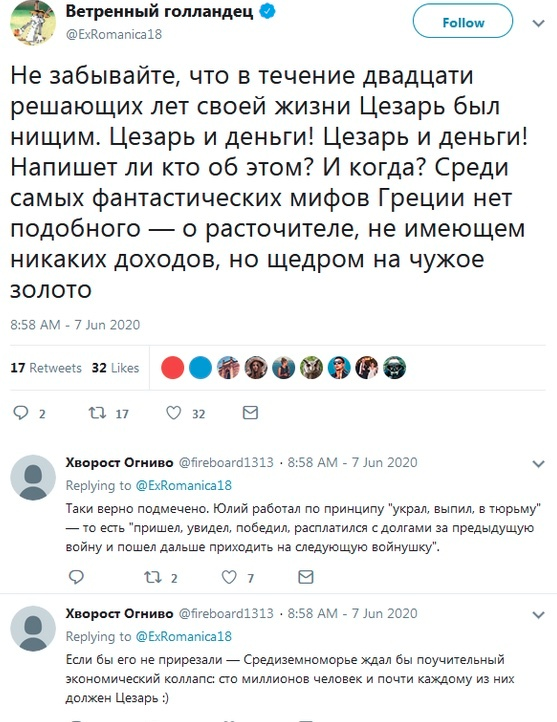
\includegraphics[scale=0.4]{Data/Caesar_and_money/1623334104151412415.png}
	\caption{Это достаточно популярное мнение. И одновременно полная чушь. Прочитайте то, что на скрине, запомните, а потом послушайте меня.
	}
	\label{fig:fabula} % Unique label used for referencing the figure in-text
	%\addcontentsline{toc}{figure}{Figure \ref{fig:placeholder}} % Uncomment to add the figure to the table of contents
\end{figure}



Да, Юлий был щедр и милостив. Он сорил деньгами. Они у него не задерживались. В моменте он не чах над златом, и всякие недалекие хипстеры даже могут посчитать его нищим, но...


Но он не только брал, но и давал деньги. И тем самым, кроме бумажек с расписками, получал друзей. То есть делал карьеру и собирал вокруг себя клиентеллу. Друзья, которые должны тебе денег, они всегда чутко прислушаются к твоим ненавязчивым просьбам, поддержат твои начинания, проголосуют где надо и всë такое. И, конечно же, он и сам много у кого занимал, и тоже чутко прислушивался, поддерживал и голосовал, это реалии тамошней политики. Если у плебеев долги это инструмент финансовый, то у аристократии это, прежде всего, инструмент политический: через долговые бумажки делалась римская политика. И без понимания этого маленького нюанса что-либо понять не представляется возможным.


А теперь кратко пройдемся по нищему Цезарю, который в финале своего двадцатилетнего путешествия стал богом.



%------------------------------------------------

\section{Первый этап: 100-63 годы (все даты до нашей эры)}\index{Lists}

\begin{figure}[h!tb]
	\centering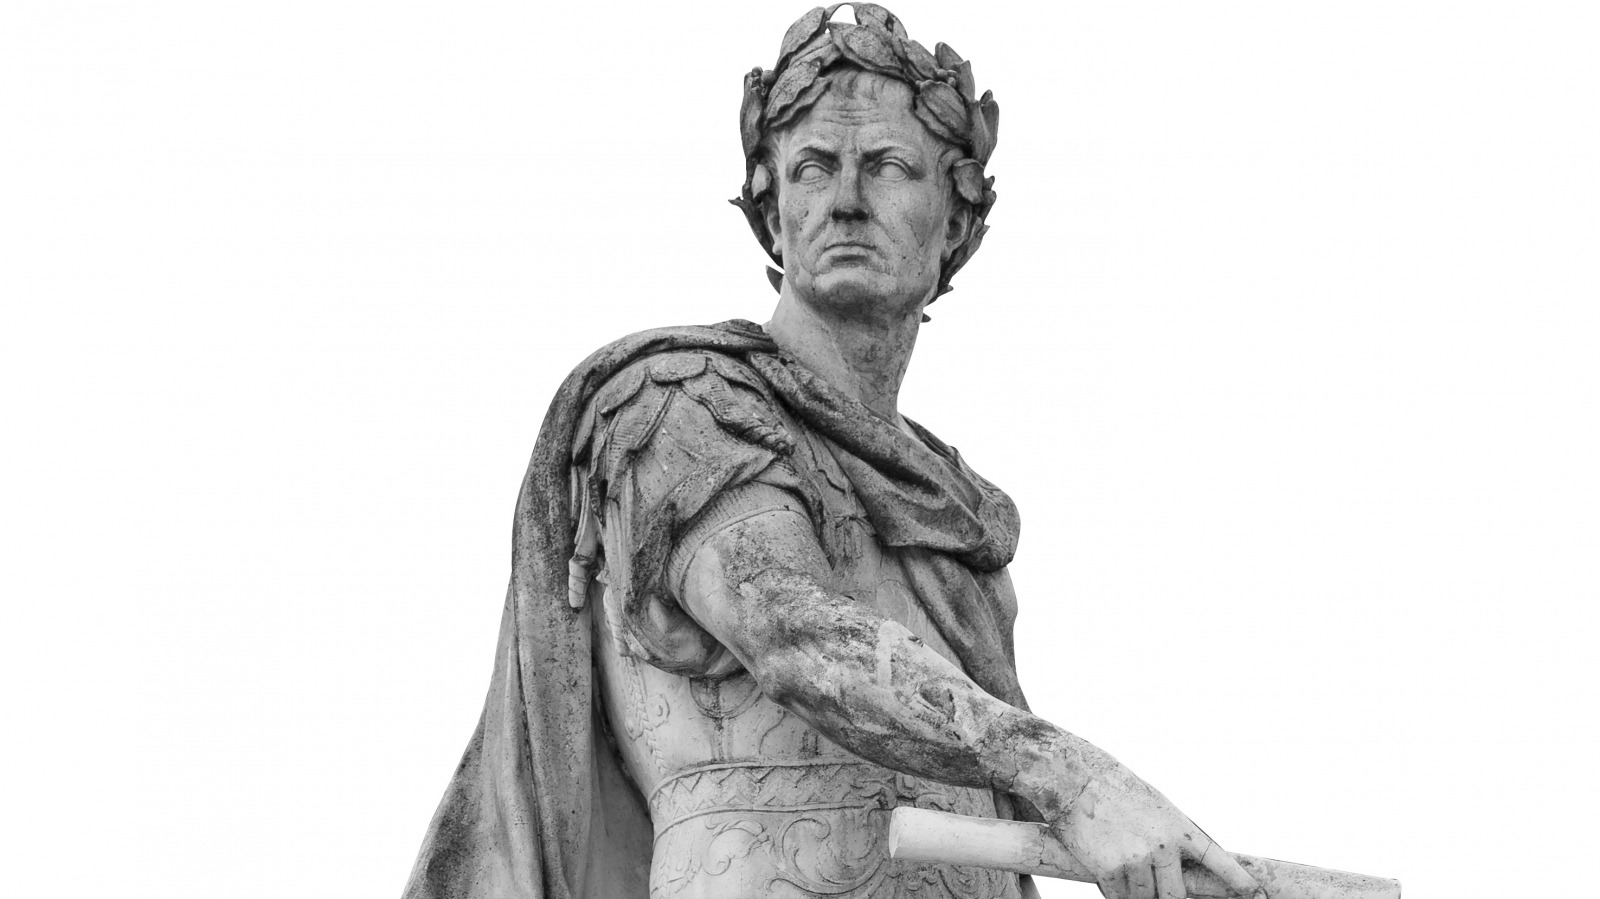
\includegraphics[scale=0.3]{Data/Caesar_and_money/16233341651643368.png}
	\caption{На пути к деньгам
	}
	\label{fig:caes1} % Unique label used for referencing the figure in-text
	%\addcontentsline{toc}{figure}{Figure \ref{fig:placeholder}} % Uncomment to add the figure to the table of contents
\end{figure}
Старт карьеры Юлия. В детстве по его семейству и друзьям семьи жестко проехался Сулла, многих там грохнули по проскрипционным спискам или лишили имущества. Поэтому стартует он с фигой в кармане и в стане просравших все полимеры популяров. А ему надо делать карьеру, причем быстро. Поэтому тут он да, влезает в долги, юлит, суетит, носится как угорелый везде где может, создает себе имя и репутацию. И тратит деньги по большей части не свои. Но большие должности — большие возможности. Поэтому своих кредиторов того периода он, судя по всему, уважил более чем, и они возврата долгов не требовали, двигая перспективного юношу вперед. Например, если взять историю с пиратами за чистую монету, то за него некие меценаты спокойно выплатили 50 талантов золотом не торгуясь (несколько сотен килограмм золота). И хоть это, скорее всего, сильно завышенная цифра, но один хрен — случай показательный. Короче говоря, тут мы можем говорить не о долгах, а о инвестициях. Юлий делал карьеру, а его друзья ему помогали, в том числе и финансово, рассчитывая отбить вложения впоследствии.


Примерно во времена восстания Спартака (73-71 г.) Цезарь, по слухам, сходится с Крассом и попадает в его команду. После этого его карьера идет в гору семимильными шагами, он просто не считает денег и очень быстро растет в должностях. При этом довольно громко продвигая популярскую повесточку. Этакий карманный оппозиционер сенатской олигархии. Учитывая, что в 70 году Красс и Помпей продавливают совместное консульство и ломают сулланскую конституцию через колено — он был очень к месту. Он поддерживает инициативы Помпея в Сенате, проходит квестуру, чинит дороги, заседает в судах, проводит игры и тратит безумное количество денег. Разменивая их на популярность в народе.


Всë это нужно было для того, чтобы быть первым в списках на по-настоящему жирные должности. Такие, которые дают реальную власть. Цезаря на этом этапе неиллюзорно прокачивали и вели, не жалея денег. Рассчитывая на то, что заняв нужное кресло, Юлий всë отработает десятикратно. Таковы реалии римской Игры Престолов.


И Цезарю везет. В 63 году умирает Великий Понтифик, и он в тяжелой борьбе занимает это вакантное кресло. Там траты вышли на ультразвук, и проиграй Цезарь выборы — его карьера вполне могла бы рухнуть. Но он победил. А Великий Понтифик, несмотря на то, что прямых именно денежных профитов должность не давала, это высшая лига. Главный жрец Республики, как-никак. Причем должность пожизненная и при этом не требующая сидеть в келье 24/7. В общем, это был успех, теперь Цезарь мог обкашливать вопросики на совсем другом уровне, а его дружба очень дорого стоила. Кредиторы Цезаря (в первую очередь это Красс) отбили свои расходы и приобрели мощный рычаг влияния на римскую политику. Причем рычаг перманетный.

\section{Второй этап: 63-59 годы}\index{Lists!Numbered List}

Если до занятия должности Понтифика Цезарь был пешкой, то теперь это фигура. Изменились и взаимоотношения с кредиторами. Теперь долги Цезаря котировались: кто ж не даст денег такому влиятельному человеку. Даже потребуй тот же Красс возврата долга, Цезарь бы просто перекредитовался у других людей и вернул деньги. А значит, и партнерство стало более равноправным. Даже несмотря на то, что долгов у Цезаря было всë ещë реально дохрена, они ему практически не мешают.


Бывает и по-другому. Например, был такой персонаж как Катилина. Который точно так же, как Цезарь, шел по карьерной лестнице, претендовал на консульство, влез в жуткие долги, поставил на карту всë, и... проиграл. И всë, гейм овер. Проиграв выборы, Катилина лишился единственного способа вернуть деньги, а значит, ему не дадут денег на следующие выборы. Более того, так как он банкрот, его затаскают по судам, заберут всë имущество и изгонят из города. Понимаете разницу? Если ты любимый народом Великий Понтифик, то никакие долги не помеха, а если ты всë просрал и банкрот, то вот тут-то и начинаются веселые игры с кредиторами и вопросы "ну как там с деньгами?". В общем, по итогу Катилина организовал заговор из таких же неудачников, основной мыслью которого было "возьмем Рим, убьем всех кто нам не нраица и аннулируем все долги". Учитывая, что для плебеев долги были реальной проблемой, многие за ним пошли. Но заговор раскрыли и разгромили. Однако я этот эпизод упомянул просто для понимания того, что ждало Цезаря при поражении.


Но Цезарь не проиграл. Наоборот, он переехал в центр города, отгрохав там виллу, избрался претором и отлично проводил время. А в 61 году уехал пропретором (военным наместником) в Испанию Дальнюю, показав там себя ещë и хорошим губернатором. За время своего пропреторства он подружился с большей частью общин региона, брал у них деньги и решал их вопросики. И воевал, кошмаря всех, кто не подчинялся и не платил. Всего за год он не только закрыл все свои долги, но и стал состоятельным человеком, который что? Что делают состоятельные люди в Риме? Правильно, они дают в долг, как мы выше говорили. Цезарь — политик, метящий на вершину, естественно, он начал обзаводиться друзьями, которые помогут ему на вершину залезть. Причем друзьями, которые ему должны.


И когда Помпей и Красс искали себе третьего человека в Триумвират, они, я полагаю, оценили в том числе и ушлость Юлия, который так быстро и ловко закрыл долги перед Крассом, да ещë и своих личных друзей начал заводить пачками. Поэтому они предлагают ему вступить с ними в альянс и избраться консулом на 59 год, чтобы уже на самом верху порешать их проблемы, ну и себя не забыть. Цезарь соглашается, прибывает в Рим и подает свою кандидатуру. За него впрягаются Помпей с Крассом, и все втроем они таки умудряются протолкать Юлия на САМЫЙ верх. Всë, дальше уже некуда, Цезарь — консул, вершина карьеры 99% всех римских политиков.


А затем, буквально за год наведя знатного шороху, Цезарь выбивает себе три провинции в проконсульство, право нанимать легионы и воевать. И оставляет римскую политику на какое-то время. Наступает третий этап его карьеры — Галльская война 

\section{Третий этап: 58-50 годы}\index{Lists!Descriptions and Definitions}

\begin{figure}[h!tb]
	\centering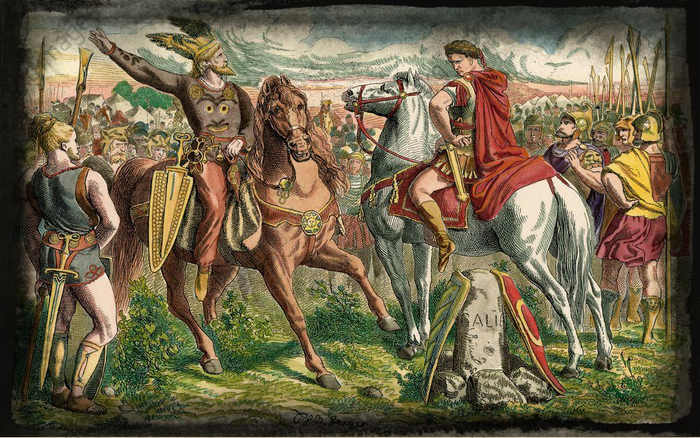
\includegraphics[scale=0.5]{Data/Caesar_and_money/1623334301188197883.png}
	\caption{Цезарь в Галлии
	}
	\label{fig:gall} % Unique label used for referencing the figure in-text
	%\addcontentsline{toc}{figure}{Figure \ref{fig:placeholder}} % Uncomment to add the figure to the table of contents
\end{figure}
Проконсулу провинции даются для управления, а не кормления. Ну, то есть бывает такое, что "наместник прибывает бедным в богатую провинцию, а убывает богатым из бедной". Явление почти рядовое. Но это долго, сложно и имеет свою цену — политические противники обязательно за это зацепятся, а их у Цезаря на этом этапе — примерно половина Рима. А Цезарь практически сходу, даже не заезжая в Иллирик, начинает набирать войска в Галлии и вести боевые действия. При этом со старта легионам кладëтся двойное жалование, а войск набирается сильно больше, чем готов был спонсировать Сенат. Цезарь, де-факто, начинает свою, частную войну в Галлии, на свои собственные деньги, осуществляя тот же сценарий, что и в Испании: обкашливать вопросики с лояльными племенами и кошмарить нелояльные, гребя деньги лопатой и с тех и с других. При этом армия Цезаря постоянно росла и более чем щедро снабжалась. К концу войны его центурионы будут в отпусках покупать себе виллы в Кампании просто чтобы деньги не залеживались. А это центурионы, легаты и выше вообще стали олигархами с личными сокровищницами. При этом галльское золото караванами текло в Рим, на раздачи народу и взятки вообще всем, кто согласен их брать. К концу войны Цезарь ЛИЧНО будет иметь клиентеллу размером со всю оптиматскую. Именно это позволит ему так хорошо начать Гражданскую войну: в Италии половина тех, кто чего-то решает — должна Цезарю денег, лол. По итогу войны он разграбил и замирил регион, став САМЫМ ВЛИЯТЕЛЬНЫМ И САМЫМ БОГАТЫМ ЧЕЛОВЕКОМ В РЕСПУБЛИКЕ, после того как Красс умер в Парфии. Его боялся даже Помпей, а денег или услуги ему должны были вообще почти все.


\begin{remark}
	Я напоминаю, мы всë ещë говорим о человеке, которого недалекие увальни считают бомжом, тонущим в долгах, лол, кек, чебурек. Я не знаю, как это комментировать. 
\end{remark}

\section{Четвертый этап: 49-44 годы}

Вот и финал Одиссеи. Переход Рубикона, начало очередной Гражданской войны. Цезарь в одну каску идет против всей Республики, которая обьявила его Врагом Отечества. И он побеждает. Он выметает Помпея из Италии, а потом громит его армии в Испании, за год стабилизируя своë положение. Попутно ему достается казна Рима, которую просто не успели вывезти, и он немедленно пускает еë на войну. Самый страшный для него 49 год, когда он реально в одно лицо пошел против всего тамошнего мира, закончился удачно.


Однако именно экономика тут стала слабым местом. По меркам человека Цезарь был безумно богат, просто невообразимо богат. Но учитывая, что ему нужно было содержать пол-Республики и воевать со второй половиной — денег очень не хватало. При этом он не может начать просто резать всех и забирать всë, это было б политическим самоубийством. Наоборот, он сейчас должен прощать и одаривать подарками. А денег мало, они утекают как песок сквозь пальцы. При этом на Востоке сидит Помпей и клепает легионы. Восток сам по себе богаче. Да ещë и партия оптиматов может не церемониться и обезжиривать своих коллег, собирая донаты на войну с Юлием. А сторонников Юлия вообще просто грабить и резать. Крч, время играет против Цезаря, его положение шатко, а денег нет. Он не беден, ещë раз, он просто ведет войну с половиной страны, а вторую половину финансирует ИЗ СОБСТВЕННОГО КАРМАНА, и тут даже Красс бы разорился к ебене матери за пару лет. 

\begin{figure}[h!tb]
	\centering
\includegraphics[scale=0.4]{Data/Caesar_and_money/16233343481189342.png}
	\caption{Аве Цезарь
	}
	\label{fig:ave} % Unique label used for referencing the figure in-text
	%\addcontentsline{toc}{figure}{Figure \ref{fig:placeholder}} % Uncomment to add the figure to the table of contents
\end{figure}


Поэтому Цезарь идет ва-банк, отплывает в Грецию и ведет там с Помпеем очень тяжелую и неудобную для себя войну. Однако, тамошние событий заканчиваются Фарсалой, где армия республиканцев наголову разбивается, и Греция падает к ногам Цезаря.


После чего он немедленно плывет в Египет и больше полугода сажает там на трон Клеопатру. А затем разбивает в Малой Азии Фарнака, перезавоевывая и этот регион. Казалось бы, что он творит, у него же гражданская война идет, а он около года тратит на Восток, занимаясь там административными вещами, пока республиканцы зализывают раны и готовятся к реваншу. В чем смысл?


А смысл в том, что восточное золото и египетский хлеб это то, что позволило опять, уже в который раз, решить финансовые проблемы, уже на уровне государства. Лояльная Клеопатра следующие годы будет неиллюзорно кормить всю Италию и снабжать еë деньгами, да и восточные царства (где Цезарь поменял всю верхушку на своих людей) не отставали. Именно они будут спонсировать все цезарианские великолепные стройки, щедрые хлебные раздачи, триумфы и реформы, они позволят ему покупать уже не отдельных политиков и даже не политические кланы, а целые социальные слои. Армия тоже получила свою долю добычи, обещанную Цезарем ещë в Галлии, и успешно закончила ему войну.


В мартовские иды 44 года Цезаря убьют. К этому моменту в государстве почти все будут Цезарем так или иначе куплены. Ветеранам он раздаст землю и выходное пособие, армия будет получать жалование, аристократы будут наперегонки делать карьеру, провинциалы получат дополнительные права, жители Рима получат свою лучшую жизнь. Куча всяких реформ проводилась, государство отдыхало от гражданской войны и готовилось к войне с Парфией (Цезаря убили за несколько недель до отплытия на Восток). А Цезарь... надо ли обьяснять?


А теперь ещë раз перечитайте на изначальном скрине эту безграмотную чушь про нищего Юлия, не знающего что такое деньги. Цезарь — гений, в том числе и финансовый. Он мастерски фехтовал легионами, он мастерски владел словом, и он мастерски использовал деньги. И он всë это использовал как оружие. Именно поэтому они, деньги, не лежали у него по сундукам. Они работали. Но какие-то ебучие хипстеры с кредитными айфонами нихуя, канешно, не поймут, и будут нам рассказывать: "гыгык, долги, нищий, смешно, салат лох, ахаха". Тьфу на них.

Ссылка на оригинал \url{https://vk.com/wall-162479647_334911}
